% LyX 1.5.5 created this file.  For more info, see http://www.lyx.org/.
% Do not edit unless you really know what you are doing.
\documentclass[english,12pt]{revtex4}
\usepackage[T1]{fontenc}
\usepackage[latin9]{inputenc}
\usepackage{nicefrac}
\usepackage{graphicx}

\makeatletter

%%%%%%%%%%%%%%%%%%%%%%%%%%%%%% LyX specific LaTeX commands.
%% Because html converters don't know tabularnewline
\providecommand{\tabularnewline}{\\}

%%%%%%%%%%%%%%%%%%%%%%%%%%%%%% User specified LaTeX commands.
%% LyX 1.5.5 created this file.  For more info, see http://www.lyx.org/.
%% Do not edit unless you really know what you are doing.



\usepackage{nicefrac}


\makeatletter

%%%%%%%%%%%%%%%%%%%%%%%%%%%%%% LyX specific LaTeX commands.
%% Because html converters don't know tabularnewline


%%%%%%%%%%%%%%%%%%%%%%%%%%%%%% User specified LaTeX commands.
%% LyX 1.5.5 created this file.  For more info, see http://www.lyx.org/.
%% Do not edit unless you really know what you are doing.



\usepackage{nicefrac}



\makeatletter

%%%%%%%%%%%%%%%%%%%%%%%%%%%%%% LyX specific LaTeX commands.
%% Because html converters don't know tabularnewline


%%%%%%%%%%%%%%%%%%%%%%%%%%%%%% User specified LaTeX commands.
%% LyX 1.5.5 created this file.  For more info, see http://www.lyx.org/.
%% Do not edit unless you really know what you are doing.



\usepackage{nicefrac}

\begin{document}


\section{Effect of the Fermi statistics on Thermal Ionization}

While simulating the ionization equilibrium in partially ionized electron-ion plasmas using Saha 
equations, the electrons are usually assumed to be an ideal Boltzmann gas.  However, the electron is a Fermion with the spin of 1/2. In practical calculations the conditions for
applicability of the Boltzmann gas model for electrons are often not satisfied, resulting in
very low accuracy. Therefore, it is worth while checking weather or not one needs to assume Boltzmann statistics for the electrons when solving the ionization equlibrium.

It appears that 
for realistic quantitative simulations this assumption is completly unnecessary, as solving the 
ionization equilibrium with the correct Fermi statistics for electrons is not a more difficult problem
than that under the incorrect assumption of Boltzmann statistics.

In a partially ionized plasma the free electron density, corrected by the effects of the Fermi statistics 
('the exchange interaction'), should be used in solving the Equation-Of-State (EOS), which is also 
directly affected by the exchange interactions. There is no need to remind that 
{\it at the given electron density} the exchange interaction increases the electron pressure and the 
internal energy density. On the other hand, in partially ionized plasmas this effect may 
be partially or even fully balanced by the electron density decrease due to the exchange interaction 
effect on the ionization equilibrium.  

{\bf Helmholtz free energy.} Consider an ionized monatomic gas with positive non-complex ions. The Helmholtz free energy,
$F=F_{ion}+F_e$, is assumed to be the total of contributions from each of the ion charge states,
$i=0$ to $i_{\max}$ (we apply Eq.(42.3) from \cite{ll} to account for these contributions), as well as the contribution from electrons:
\begin{equation}\label{freeenergy}
F=-T
\sum_{i=0}^{i_{max}}{
N_i\log\left[g_i
             \frac{eV}{N_i}\left(\frac{MT}{2\pi \hbar^2}\right)^{3/2}\exp \left(-\sum_{j=0}^{i-1}\frac{I_j}T \right)\right]}+F_e,
\end{equation}  
where $N_i=n_iV$ is the total number of ions in the charge state $i$ in the volume V and
$I_j$ ($j = 0, 1, 2, \dots$) is the energy needed to ionize an atom or ion from the charge state $j$ to the charge state $j+1$ (the ionization potential).

{\bf Ionization equilibrium: formulation of the problem.} Now we formulate the requirement for the
ionization equilibrium with respect to the reaction $(i)\leftrightarrow(i+1)+e$ for each ion charge state, $i$.
The Helmholtz free energy is a minimum at the equilibrium set of $N_i$ and $N_e$. Therefore, the total
derivative of F with respect to $N_e$ should be zero:
\begin{equation}
\frac{\partial F}{\partial N_e} + \frac{d N_i}{d N_e} \frac{\partial F}{\partial N_i} +
\frac{d N_{i+1}}{d N_e} \frac{\partial F}{\partial N_{i+1}} = 0.
\end{equation}
For the reaction under
consideration, the increments in the particle numbers should be 
related as follows: $dN_{i}=-dN_{i+1}=-dN_e$.
Therefore the requirement, $dF/dN_{i}-dF/dN_{i+1}-dF/dN_e=0$, gives:
\begin{equation}\label{equili}
-T\log\left[\frac{g_{i}}{N_{i}} e^{-\sum_{j=0}^{i-1}I_j/T}\right] + T\log\left[\frac{g_{i+1}}{N_{i+1}} e^{-\sum_{j=0}^{i}I_j/T}\right]-\mu_e=0,
\end{equation}
where we applied the definition of the chemical potential, $\mu=(\partial F/\partial N)_{T,V}$, to the electron gas.
The solution of the ionization equilibrium, therefore, reads:
\begin{equation}
N_{i+1}/g_{i+1}=(N_i/g_i)e^{(-\mu_e-I_i)/T},
\end{equation}
or, applying this recursively:
\begin{equation}\label{saharecursive}
N_{i}/g_{i}=(N_0/g_0)e^{(-i\mu_e-\sum_{j=0}^{i-1}I_j)/T}=N_0g_0(g_e)^ie^{-\sum_{j=0}^{i-1}I_j/T},\,\,\,g_e=e^{-\mu_e/T},
\end{equation}
where $g_e$ is the effective "statistical weight" of a free electron.
Indeed, the effective statistical weight of i electrons combined with an ion in the charge state, i, is the
product of statistical weights for each of the particles under consideration, $(g_e)^i g_i$, in accordance with Eq.(\ref{saharecursive}).

In the limiting case of $g_e\gg1$ 
(a Boltzmann gas of electrons with large negative value of $\mu_e$), $g_e$ might be interpreted as the
large number of elementary quantum states the detached electron can occupy, which facilitates the ionization by resulting in a higher total probability for 
the ionized state. In the opposite limiting case of a degenerate Fermi gas of electrons, the positive chemical potential, $\mu_e>0$, 
tends to the Fermi energy $E_F$, which in
this limiting case is much greater than the temperature. Accordingly, the exponentially low value of $g_e=e^{-E_F/T}$ in this case means the low 
probability for an electron to jump from a bound state with negative energy to a free state above the threshold of the positive Fermi energy.  

{\bf Partition function and electron density}. We now introduce the ion partition function, $p_i=N_i/N_a$, $N_a$, being 
the total number of atoms. Since the partition function is normalized by unity,
we have:
\begin{equation}
p_i=\frac{g_i(g_e)^ie^{-E_i/T}}S,
\end{equation}
where we introduced the statistical sum:
\begin{equation}
S=\sum_{i=0}^{i_{max}}\left[g_i(g_e)^ie^{-E_i/T}\right],
\end{equation}
as well as the total ionization energy spent to ionize the atom to the state $i$:
\begin{equation}
E_i=\sum_{j=0}^{i-1}I_j.
\end{equation}
Introducing the averaging operator acting on an arbitrary function of the ion charge number, $\langle f_i\rangle=\sum p_if_i$, and assuming quasi-neutrality, $N_e = \sum{i N_i}$, we
obtain the expression for the electron density:
\begin{equation}\label{zavr}
Z=N_e/N_a=\langle i\rangle.
\end{equation}
On the other hand, for given $T$ and $n_A=N_a/V$ the electron concentration may be found as a function of $g_e(=e^{-\mu_e/T})$.
Now we assume that the electron form an ideal Fermi gas.
This assumption immediately gives us another relationship between the electron density and $g_e$ (see Eq.(56.5) from \cite{ll}):
\begin{equation}\label{zfe}
Z=g_{e1}{\rm Fe}_{1/2}(g_e).
\end{equation}
The coupled equations (\ref{zavr}) and (\ref{zfe}) are used below to solve $Z$ and $g_e$. Here
\begin{equation}
g_{e1}(T,N_a/V)=\frac{2V}{N_a}\left(\frac{m_eT}{2\pi \hbar^2}\right)^{3/2}
\end{equation}
is a value such that in the {\it Boltzmann} electron gas $g_e = g_{e1}/Z$ would hold. ${\rm Fe}_\nu(g_e)$ is the Fermi function:
\begin{equation}
{\rm Fe}_\nu(g_e)=\frac1{\Gamma(\nu+1)}\int{\frac{x^\nu dx}{g_ee^x+1}},
\end{equation}
where $\Gamma$-function is introduced as usuall: $\Gamma(\nu+1)=\nu \Gamma(\nu),\,\Gamma(1/2)=\pi^{1/2}$.
Below we use the following auxiliary functions:
\begin{equation}
R^-(g_e)=\frac{{\rm Fe}_{-1/2}(g_e)}{{\rm Fe}_{1/2}(g_e)} and \qquad
R^+(g_e)=\frac{{\rm Fe}_{3/2}(g_e)}{{\rm Fe}_{1/2}(g_e)}.
\end{equation}
Detailed discussion on the Fermi functions is delegated to the Appendix.

{\bf To solve the ionization equilibrium} for the given $T$ and $n_a=N_a/V$, one needs to solve $g_e$ from equation $G(g_e)=0$, 
$G(g_e)=\langle i\rangle-g_{e1}{\rm Fe}_{1/2}(g_e)$, which is obtained by means of excluding $Z$ from Eqs.(\ref{zavr},\ref{zfe}). 
It may be solved using the Newton-Rapson iterations with any trial value, $\log(g_e)_{old}$, the improved value, $\log(g_e)_{new}$, 
is obtained from the equation as follows:
\begin{equation}\label{iter}
\log(g_e)_{new}=%\log(g_e)_{old}-\frac{G((g_e)_{old})}{G^\prime((g_e)_{old})}=
\log(g_e)_{old}-\frac{\langle i\rangle-g_{e1}{\rm Fe}_{1/2}((g_e)_{old})}{
\langle i^2\rangle-\langle i\rangle^2+ Z R^-((g_e)_{old}) },
\end{equation}
where the derivative $g_eG^\prime$, which should stand in the denominator of 
Eq.(\ref{iter}), is derived using the easy-to-check equations as follows:
\begin{equation}
g_e\frac{d{\rm Fe}_\nu(g_e)}{dg_e}=-{\rm Fe}_{\nu-1}(g_e),
\end{equation}
and for any set of values in the charge states, $f_i$:
\begin{equation}
g_e\frac{\partial\langle f_i\rangle}{\partial g_e}=\langle if_i\rangle-\langle f_i\rangle\langle i\rangle.
\end{equation}

We see that to solve iterations in Eq.(\ref{iter}) for Fermi gas of electrons is not a
more computationally intense problem compared to the same procedure by assuming electrons 
to be a Boltzmann gas. In the latter case, $g_e \to +\infty$, we have ${\rm Fe}_\nu(g_e) \approx 1/g_e$
(see Eq.(\ref{feboltzmann}) below) and $g_e \approx g_{e1}/Z$, which allows us to iterate Eq.(\ref{iter})
as a somewhat simpler equation for $Z$:
$\log (Z_{new})=\log(Z_{old})+(\langle i\rangle-Z_{old})/(Z_{old}+\langle i^2\rangle-\langle i\rangle^2)$. However in any case, the most cumbersome computations 
while solving Eq.(\ref{iter}) for a Fermi gas, or the equation for $Z$ for a Boltzmann gas, is in explicitly calculating the 
numerous partition functions for many charge
states and excitation levels. Compared with these bulk computations, the presence of the Fermi functions in Eq.(\ref{iter}), which may be tabulated 
for all interesting cases of $\nu=-1/2,1/2,3/2$, % as well as a single inverse function, ${\rm Fe}^{-1}_{1/2}$ 
does not matter at all.

Therefore, we 
do not see any reason for applying the assumption of a Boltzmann electron gas in modelling the ionization equilibrium
in real dense plasmas.

{\bf Derivatives along the ionization curve.}
Taking differential of the equation of ionization equilibrium, $G=0$, one gets the equation relating the differentials
of different variables along the curve of ionization equilibrium:
\begin{equation}\label{diffge}
\frac{dg_e}
{g_e}
\left(
\langle i^2\rangle-Z^2+ZR^-(g_e)
\right)+\frac{dT}{T^2}
\left(\langle iE_i\rangle-\langle E_i\rangle Z)\right)=\left(\frac32\frac{dT}{T}+\frac{dV}V\right)Z,
\end{equation}
here we substitute wherever possible $Z$ for $\langle i\rangle$ and $g_{e1}{\rm Fe}_{1/2}(g_e)$.
Accordingly, the differential of $Z$ is:
\begin{equation}\label{diffz}
dZ=\left(\frac32\frac{dT}{T}+\frac{dV}V-\frac{R^-(g_e)dg_e}{g_e}\right)Z.
\end{equation}

{\bf Estimate the effect of the Fermi statistics on the ionization degree.}
Eqs.(\ref{diffge},\ref{diffz}) allow us to evaluate the effect of electron Fermi statistics on ionization.
From Eq.(\ref{feboltzmann}) one can
see that for large $g_e$ (Boltzmann gas) the equation, $G(g_e)=0$, reduces to $\langle i\rangle-g_{e1}/g_e=\delta_{\rm Fe}$,
where $\delta_{\rm Fe}$ is a small negative correction to the Fermi function at $g_e \to \infty$:
\begin{equation}\label{feboltzmann}
{\rm Fe}_\nu(g_e)=\frac{1}{\Gamma(\nu+1)} \int \frac{x^\nu dx}{g_e e^x + 1} =
\frac{1}{\Gamma(\nu+1)} \int \frac{x^\nu dx}{g_e e^x} + \delta_{\rm Fe} = \frac{1}{g_e} + \delta_{\rm Fe}.
\end{equation}
%Considering $\delta_{\rm Fe}$ negligible, one can find $g_e=g_{e1}/Z$ from Eq.(\ref{zfe})

Assuming $\delta_{\rm Fe}$ to be a small increment in the right hand side of Eqs.(\ref{diffge},\ref{diffz}), and by
finding $dg_e/\delta_{\rm Fe}$ from Eq.(\ref{diffge}) at $dV=dT=0$ and then finding $dZ/\delta_{\rm Fe}$ from Eq.(\ref{diffz}) gives:
\begin{equation}
\delta Z=Z\delta_{\rm Fe}\frac{\langle i^2\rangle-Z^2}{\langle i^2\rangle-Z^2+Z}. 
\end{equation}
The correction is negative as long as $\delta_{\rm Fe}$ is negative. Thus, due to the Fermi gas effects for detached electrons, the ionization degree is
always lower than that predicted by the Saha equilibrium equations under the assumption of a Boltzmann electron gas.

This effect should be accounted for while
treating the effect of the Fermi statistics for electrons in the equation of state. Specifically, {\it at constant electron density} the exchange interactions 
between the electrons increases the electron pressure, but in the partially ionized plasma the magnitude (if not the sign!) of this effect can be  
compromised by the pressure reduction due to the decrease in the electron density. 

{\bf Plasma thermodynamics and Equation-Of-State.} Now we substitute the ion partition function into Eq.(\ref{freeenergy}). After some algebra we obtain:
\begin{equation}\label{equile}
F = -TN_a\log\left[\frac{eV}{N_a}\left(\frac{MT}{2\pi \hbar^2}\right)^{3/2}\right]-TN_a\log S +\Omega_e,
\end{equation}
the thermodynamic potential $\Omega_e=F_e -\mu_eZN_a$ for Fermi gas of electrons is given by Eq.(56.6) from \cite{ll}:
\begin{equation}
\Omega_e = -[g_{e1}N_a]T{\rm Fe}_{3/2}(g_e),
\end{equation}
the product in the square brackets, being actually independent of $N_a$, because $g_{e1}\sim N_a^{-1}$ Eq.(\ref{equile}), provides the free energy in the case of
local thermodynamic equilibrium with the first term being the contribution from the ion translational energy. This term may be written as the function of the ion 
temperature, in the case the latter differs from the electron temperature. Unless the ion-ion interaction is taken into account, this first term gives the contributions 
of $n_aT_i$ and $3n_aT_i/2$ to the total plasma pressure and total energy density correspondingly. The second term is
the Boltzmann distribution of ions over the ionization and excitation states, expressed in terms of the statistical sum. Finally, the electron gas with the
variable particle number gives the contribution of $\Omega_e$ instead of $F_e$. 

While differentiating Eq.(\ref{equile}) with respect to $T$ and $V$, it is important that the derivatives
by $g_e$ from the second and third terms cancel 
each other: $g_e(\partial \log S/\partial g_e)=\langle i\rangle=Z$ and $-g_eg_{e1}{\rm Fe}^\prime_{3/2}(g_e)=g_{e1}{\rm Fe}_{1/2}=Z$. That is why for the internal energy density, 
${\cal E}$, and for the pressure we find:
\begin{equation}
{\cal E} = -\frac{T^2}V\left(\frac{\partial}{\partial T}\left(\frac F T\right)\right)=
{\cal E}_i+{\cal E}_e,\qquad{\cal E}_i=\frac32Tn_a,
\qquad{\cal E}_e=n_a\left[\frac32TZR^+(g_e)+\langle E_i\rangle\right],
\end{equation}
\begin{equation}
P = -\frac{\partial F}{\partial V}=P_i+P_e,\qquad
P_i = n_aT,\qquad
P_e = n_aTZR^+(g_e).
\end{equation}

However, while calculating the second order thermodynamic derivatives, like the specific heat, the derivatives of $g_e$ essentially sophisticate the 
calculations. The result may be expressed in terms of covariances: $\langle\delta^2i\rangle=\langle(i-Z)^2\rangle$, $\langle\delta^2E\rangle=\langle(E_i-\langle E_i\rangle)^2 \rangle$ and 
$\langle\delta i\delta E\rangle=\langle(E_i-\langle E_i\rangle)(i-Z)\rangle$. In a similar way one can find the specific heat in an isochoric process, per the unit of volume:
\begin{equation}
C_{Ve}=\frac{\partial {\cal E}_e}{\partial T}=n_a\left[\frac{\langle\delta^2E\rangle}{T^2}+\frac{15}4ZR^+
-\frac{\left(\frac32Z-\frac{\langle\delta E\delta i\rangle}T\right)^2}{\langle\delta^2i\rangle+ZR^-}\right],
\end{equation}
the temperature derivative of pressure:
\begin{equation}
\frac {\partial P_e}{\partial T}=n_aZ\left[\frac52 R^+ -\frac{\frac32Z-\frac{\langle\delta E\delta i\rangle}T}{\langle\delta^2i\rangle+ZR^-}\right],
\end{equation}
as well as the isothermal compressibility:
\begin{equation}
V\frac{\partial P_e}{\partial V}=-\frac{Z^2n_aT_e}{\langle\delta^2i\rangle+ZR^-}.
\end{equation}
For simplicity in the above equations, the contributions due to ion translational motions,
\begin{equation}
C_{Vi}=\frac32n_a, \qquad
\frac{\partial P_i}{\partial T}=n_a, \qquad
V\frac{\partial P_i}{\partial V}=-n_aT,
\end{equation}
are omitted.

The speed of sound, $C_s$ is defined in terms of the adiabatic comressibility (at constant entropy), $C_s^2=\left(\frac{\partial P}{\partial \rho}\right)_{\rm ad}$, which
may be parametrized in terms of 'effective polytropic index', $\gamma$, such that 
$\gamma\frac{P}\rho=\left(\frac{\partial P}{\partial \rho}\right)_{\rm ad}$, herewith $\rho$ is the mass density. To calculate this, one can take Eq.(3.72) from 
\cite{drake}, 
$$
\left(\frac{\partial P}{\partial \rho}\right)_{\rm ad}=\left(\frac{\partial P}{\partial \rho}\right)_T-
\frac{\rho}{C_V}\left[
\left( \frac{\partial({\cal E}/\rho)}{\partial \rho}\right)_T-\frac{P}{\rho^2}\right]\left(\frac{\partial P}{\partial \rho}\right)_T.
$$
Note that in \cite{drake} both the internal energy and the specific heat are related per a unit of mass, while we relate them to the unit of volume.  
Now we apply the thermodynamic identity as follows:
\begin{equation}
\left( \frac{\partial ({\cal E}/\rho)}{\partial \rho} \right)_{T} - \frac{P}{\rho^2} =
-\frac{T}{\rho^2} \left( \frac{\partial P}{\partial T} \right)_{\rho},
\end{equation}
which gives
\begin{equation}
\gamma = \frac{\rho}{P} \left( \frac{\partial P}{\partial \rho} \right)_T +
\left( \frac{\partial P}{\partial T} \right)^2_\rho \frac{T}{C_V P}.
\end{equation}
Note that in the last three equations we denote the derivative at constant $V$ as that at constant $\rho$ and used the derivatives over $\rho$ instead of those over $V$:
 $V\frac\partial{\partial V}=-\rho\frac\partial{\partial \rho}$.
\section{Madelung approximation of electrostatic energy}
{\bf Coulomb interactions} we account within the Madelung approximation. The extra term in the free energy which accounts for the
electrostatic energy of each of the ions in the charge state $i$ coupled with i electrons, the latter being uniformly
distributed over the "iono-sphere"
(see Eq.(3.50) in \cite{drake}):
\begin{equation}\label{fterm}
F_M=-\frac{9}{10} \frac{q_e^2}{r_{iono}} \sum_{i=0}^{i_{max}} i^2 N_i,\qquad
r_{iono} = \left( \frac{4 \pi}{3} n_a \right)^{-\frac13}.
\end{equation}
Accordingly, in the requirement of the ionization equilibrium, $\partial F/\partial N_i - \partial F/\partial N_{i+1} - \partial F/\partial N_e = 0$ (with respect to the reaction $(i)\leftrightarrow(i+1)+e$),
the term $\partial F_{M}/\partial N_i -\partial F_{M}/\partial N_{i+1}$ will 
give the contribution of $\frac{9}{10} \frac{(2i+1)q_e^2}{r_{iono}}$ into the left hand side:
\begin{equation}
-T \log \left[ \frac{g_i}    {N_i}     e^{\sum_{j=0}^{i-1} I_j/T} \right] - \frac{9}{10} \frac{i^2     q_e^2}{r_{iono}}
+T \log \left[ \frac{g_{i+1}}{N_{i+1}} e^{\sum_{j=0}^i     I_j/T} \right] + \frac{9}{10} \frac{(i+1)^2 q_e^2}{r_{iono}}
-\mu_e = 0.
\end{equation}
The solution of the ionization equilibrium, hence, reads:
\begin{equation}
\frac{N_{i+1}}{g_{i+1}} = \frac{N_i}{g_i} \exp\left(-\frac1T \left(I_i - \frac{9}{10} \frac{(2i+1) q_e^2}{r_{iono}} + \mu_e \right)\right),
\end{equation}
or, applying this recursively and reducing the sum $\sum_{j=0}^{i-1} (2j+1) = i^2$,
\begin{equation}\label{pfM}
\frac{N_i}{g_i}=\frac{N_0}{g_0}(g_e)^i \exp \left( \frac{9}{10} \frac{i^2 q_e^2}{T r_{iono}} -\frac{\sum_{j=0}^{i-1}I_j}T \right) .
\end{equation}
This may be interpreted as the ionization potential lowering which results from the Coulomb interaction:
each of the potentials, $I_i$, is reduced by $\frac{9}{10} \frac{(2i+1)q_e^2}{r_{iono}}$.
Energy of the ion of the charge state $i$ is $E_i^* = \sum_{j=0}^{i-1}I_j - \frac{9}{10} \frac{i^2 q_e^2}{r_{iono}}$.
This effect shifts the ionization equilibrium towards higher ionization degrees, for a given temperature and atomic density.

The common multiplier, $\frac{N_0}{g_0}$, in each of Eqs.(\ref{pfM}) may be also represented as $\frac{N_a}{S}$.
From the normalization condition, $\sum N_i = N_a$, we find that $S$ is a statistical sum:
\begin{equation}
S=\sum_{i=0}^{i_{max}} g_i (g_e)^i \exp\left(-\frac{E_i^*}T\right),
\end{equation}
so that:
\begin{equation}\label{ni}
p_i = \frac{N_i}{N_a} = \frac{1}S g_i (g_e)^i \exp \left( -\frac{E_i^*}T \right).
\end{equation}

The full Helmholtz free energy now includes the contribution of the electrostatic field energy as in Eq.(\ref{fterm}):
\begin{equation}\label{fe1}
F=-T
\sum_{i=0}^{i_{max}}{
N_i\log\left[g_i
  \frac{eV}{N_i}\left(\frac{MT}{2\pi \hbar^2}\right)^{3/2}\exp \left(-\sum_{j=0}^{i-1}\frac{I_j}T \right)\right]}+F_e
  -\frac{9}{10} \sum_{i=0}^{i_{max}} N_i \frac{i^2 q_e^2}{r_{iono}}.
\end{equation}  

With the ion partition functions as in Eq.(\ref{ni}) one can rewrite Eq.(\ref{fe1}) in the following form:
\begin{equation}\label{ffullm}
F = -TN_a\log\left[\frac{eV}{N_a}\left(\frac{MT}{2\pi \hbar^2}\right)^{3/2}\right]-TN_a\log S + \Omega_e, 
\end{equation}
where, again, $\Omega_e = F_e - \mu_e N_a \sum i p_i = F_e - \mu_e N_a \langle i \rangle $.

{\bf Differentials along the curve of the ionization equilibrium} obey the equation as follows:
\begin{equation}\label{diffstruct}
A_{g_e} \frac{dg_e}{g_e} = A_V \frac{dV}{V} + A_T \frac{dT}{T},
\end{equation}
\begin{equation}
A_{g_e} = \langle \delta^2 i \rangle + ZR^-(g_e), \qquad
A_T     = \frac32 Z - \frac{\langle \delta i \delta E^*_i \rangle}{T}, \qquad
A_V     = Z + L \langle \delta(i^2) \delta i \rangle,
\end{equation}
where $L$ can be expressed either in CGS units or as it appears in the code:
\begin{equation}
L_{CGS}   = \frac{3}{10} \frac{q_e^2}{T r_{iono}}, \qquad
L = \frac35 \frac{Ry[eV]}{T[eV] r_{iono}[a]},
\end{equation}
where $Ry[eV]$ denotes the Rydberg constant expressed in electron-volts, and
$r_{iono}[a]$ stands for the ionosphere radius expressed in the units
of Bohr radius.

Again, we express the result in terms of covariances,
$\langle \delta a \delta b \rangle = \langle (a - \langle a \rangle) (b - \langle b \rangle) \rangle$,
and mean values which are now being calculated
using the modified partition functions.
Differentiation of mean values which is necessary for derivation of the above equation on
differentials is not a complicated problem with the following formula:
\begin{equation}
d \langle f_i \rangle = \left\langle \delta f_i \delta\left( \frac{dp_i}{p_i} \right) \right\rangle,
\end{equation}
where $f_i$ is a function of the only argument $i$, for example, $iE_i$ or $i^2+i$.

{\bf Plasma thermodynamics and Equation-Of-State.} 
While differentiating Eq.(\ref{ffullm}) with respect to $T$ and $V$, again, we see that the derivatives
by $g_e$ from the second and third terms cancel 
each other: $g_e(\partial \log S/\partial g_e)=\langle i\rangle=Z$,
that is evident from $d \log S = \langle d (\log p_i) \rangle$,
and $-g_eg_{e1}{\rm Fe}^\prime_{3/2}(g_e)=g_{e1}{\rm Fe}_{1/2}=Z$.
That is why for the internal energy density,
${\cal E}$, and for the pressure, $P$, we find the general expressions
as follows:
\begin{equation}\label{generalE}
{\cal E} = -\frac{T^2}V\left(\frac{\partial}{\partial T}\left(\frac F T\right)\right)=
{\cal E}_i+{\cal E}_e,\qquad{\cal E}_i=\frac32Tn_a,\qquad
{\cal E}_e = n_a\left[ \frac32 T Z R^+ + \langle E \rangle \right],
\end{equation}
\begin{equation}\label{generalP}
P = -\frac{\partial F}{\partial V}=P_i+P_e,\quad
P_i = n_aT,\quad
P_e = n_a \left[ T ZR^+ - V \langle \frac{\partial E}{\partial V} \rangle \right],
\end{equation}
where we assume $E=E(V)$.

In the above equations we add the Madelung corrections into the energy of the electron gas, ${\cal E}_e$, and
into the pressure of electrons, $P_e$, because those corrections are controlled by the electron temperature.

The thermodynamic derivatives can also be expressed in a general form for $E=E(V)$.
In such a way one can find the specific heat in isochoric process, per the unit of volume:
\begin{equation}\label{generalCv}
C_{Ve}=\frac{\partial {\cal E}_e}{\partial T}=n_a\left[\frac{\langle\delta^2 E \rangle}{T^2}+\frac{15}4ZR^+
-\frac{\left(\frac32Z-\frac{\langle\delta E \delta i\rangle}T\right)^2}{\langle\delta^2i\rangle+ZR^-}\right],
\end{equation}
the temperature derivative of pressure:
\begin{equation}\label{generalPT}
\frac {\partial P_e}{\partial T}=
n_a\left[
	\frac52 Z R^+ -
	\left( Z+\frac{V}{T} \langle \delta \frac{\partial E}{\partial V} \delta i \rangle \right)
		\frac{\frac32Z-\frac{\langle\delta E \delta i\rangle}T}{\langle\delta^2i\rangle+ZR^-} -
	\frac{V}{T^2} \langle \delta \frac{\partial E}{\partial V} \delta E \rangle
\right],
\end{equation}
as well as the isothermal compressibility:
\begin{equation}\label{generalCompr}
V\frac{\partial P_e}{\partial V}=
n_a T \left[ -\frac{\left(Z + \frac{V}{T} \langle \delta i \delta \frac{\partial E}{\partial V} \rangle \right)^2}
{\langle \delta^2 i \rangle + ZR^-} +
\frac{V^2}{T^2} \langle \delta^2 \frac{\partial E}{\partial V} \rangle -
\frac{V^2}{T} \langle \frac{\partial^2 E}{\partial V^2} \rangle
\right].
\end{equation}
Again, for simplicity in the above equations the contributions due to ion translational motions,
\begin{equation}
C_{Vi}=\frac32n_a, \qquad
\frac{\partial P_i}{\partial T}=n_a, \qquad
V\frac{\partial P_i}{\partial V}=-n_aT,
\end{equation}
are omitted.

To apply the Madelung theory we calculate the first and the second partial derivatives
of the energy levels over volume:
\begin{equation}
E = E^*_i, \qquad
\frac{V}{T} \frac{\partial E}{\partial V} = L i^2, \qquad
\frac{V^2}{T} \frac{\partial^2 E}{\partial V^2} = -\frac43 L i^2,
\end{equation}
and substitute them into the general formulas for the thermodynamic variables
and the thermodynamic derivatives:
\begin{eqnarray}
\label{madE}
{\cal E}_e &=& n_a\left[ \frac32 T Z R^+ + \langle E^*_i \rangle \right], \\
\label{madP}
P_e &=& n_aT ( ZR^+ - L \langle i^2 \rangle ), \\
\label{madCv}
C_{Ve} = \frac{\partial {\cal E}_e}{\partial T} &=& n_a\left[\frac{\langle\delta^2E^*_i\rangle}{T^2}+\frac{15}4ZR^+
-\frac{\left(\frac32Z-\frac{\langle\delta E^*_i\delta i\rangle}T\right)^2}{\langle\delta^2i\rangle+ZR^-}\right], \\
\label{madPT}
\frac {\partial P_e}{\partial T} &=&
n_a\left[
	\frac52 Z R^+ -
	(Z+L \langle \delta(i^2) \delta i \rangle)
		\frac{\frac32Z-\frac{\langle\delta E^*_i\delta i\rangle}T}{\langle\delta^2i\rangle+ZR^-} -
	L \frac{\langle \delta E^*_i \delta(i^2) \rangle}T
\right], \\
\label{madCompr}
V\frac{\partial P_e}{\partial V} &=&
n_a T \left[ -\frac{(Z + L \langle \delta(i^2) \delta i \rangle)^2}{\langle \delta^2 i \rangle + ZR^-} +
L \left( \frac43 \langle i^2 \rangle + L \langle \delta^2(i^2) \rangle \right) \right].
\end{eqnarray}

Following is the table showing the values of $Z$ calculated for Xenon
at various electron temperatures
(given in electron-volts -- the value of $k_{B}T_{e}$, where $k_{B}$
is in eV/K) and heavy particle concentrations (given in number of
particles per $cm^{3}$). "no" columns contain the same values
calculated without Coulomb interation taken into account.

\begin{center}
\begin{tabular}{|c||c|c|c|c|c|c|c|c|c|c|c|c|}
\hline
Na[$1/cm^3$] & \multicolumn{2}{|c|}{$10^{18}$} & \multicolumn{2}{|c|}{$10^{19}$} & \multicolumn{2}{|c|}{$10^{20}$} & \multicolumn{2}{|c|}{$10^{21}$} & \multicolumn{2}{|c|}{$10^{22}$} & \multicolumn{2}{|c|}{$10^{23}$}\tabularnewline
\hline
Te[eV] & no & Mad & no & Mad & no & Mad & no & Mad & no & Mad & no & Mad\tabularnewline
\hline
\hline
   5. &     3.4 &     3.4 &     2.8 &     3.0 &     2.2 &     2.5 &     1.3 &     1.9 &     0.6 &     1.4 &     0.2 &     2.9\tabularnewline
\hline
  10. &     6.3 &     6.4 &     5.2 &     5.4 &     4.1 &     4.6 &     3.0 &     3.7 &     1.7 &     3.2 &     0.7 &     3.9\tabularnewline
\hline
  15. &     7.3 &     7.3 &     6.9 &     6.9 &     5.9 &     6.3 &     4.4 &     5.4 &     2.7 &     4.6 &     1.1 &     4.8\tabularnewline
\hline
  20. &     9.2 &     9.3 &     7.7 &     7.9 &     6.9 &     7.1 &     5.6 &     6.5 &     3.6 &     5.7 &     1.6 &     5.6\tabularnewline
\hline
  25. &    11.8 &    12.0 &     9.4 &     9.7 &     7.6 &     8.0 &     6.5 &     7.1 &     4.5 &     6.5 &     2.1 &     6.2\tabularnewline
\hline
  30. &    13.8 &    14.0 &    11.5 &    11.9 &     8.9 &     9.5 &     7.1 &     7.8 &     5.4 &     7.0 &     2.6 &     6.7\tabularnewline
\hline
  35. &    15.7 &    15.9 &    13.3 &    13.7 &    10.4 &    11.3 &     7.8 &     8.9 &     6.0 &     7.6 &     3.1 &     7.2\tabularnewline
\hline
  40. &    17.2 &    17.4 &    14.9 &    15.3 &    12.1 &    12.9 &     8.7 &    10.2 &     6.6 &     8.3 &     3.6 &     7.8\tabularnewline
\hline
  45. &    18.1 &    18.2 &    16.4 &    16.7 &    13.4 &    14.2 &     9.9 &    11.6 &     7.1 &     9.2 &     4.1 &     8.5\tabularnewline
\hline
  50. &    19.0 &    19.2 &    17.4 &    17.7 &    14.7 &    15.5 &    11.1 &    12.9 &     7.6 &    10.3 &     4.6 &     9.3\tabularnewline
\hline
  55. &    20.5 &    20.7 &    18.1 &    18.4 &    15.9 &    16.7 &    12.3 &    14.0 &     8.2 &    11.4 &     5.0 &    10.1\tabularnewline
\hline
  60. &    22.0 &    22.2 &    19.0 &    19.3 &    16.9 &    17.5 &    13.3 &    15.1 &     8.8 &    12.4 &     5.5 &    11.0\tabularnewline
\hline
  65. &    23.3 &    23.5 &    20.1 &    20.6 &    17.6 &    18.1 &    14.3 &    16.0 &     9.6 &    13.4 &     5.9 &    11.9\tabularnewline
\hline
  70. &    24.4 &    24.6 &    21.4 &    21.9 &    18.2 &    18.8 &    15.2 &    16.8 &    10.4 &    14.3 &     6.2 &    12.7\tabularnewline
\hline
  75. &    25.3 &    25.4 &    22.6 &    23.0 &    19.0 &    19.7 &    16.1 &    17.5 &    11.2 &    15.1 &     6.6 &    13.5\tabularnewline
\hline
  80. &    25.7 &    25.7 &    23.6 &    24.0 &    19.8 &    20.7 &    16.8 &    18.0 &    12.0 &    15.8 &     6.9 &    14.2\tabularnewline
\hline
  85. &    25.9 &    25.9 &    24.5 &    24.8 &    20.8 &    21.8 &    17.4 &    18.6 &    12.7 &    16.5 &     7.3 &    14.9\tabularnewline
\hline
  90. &    25.9 &    25.9 &    25.1 &    25.3 &    21.9 &    22.7 &    17.9 &    19.2 &    13.5 &    17.0 &     7.7 &    15.5\tabularnewline
\hline
  95. &    26.0 &    26.0 &    25.5 &    25.6 &    22.8 &    23.6 &    18.5 &    20.0 &    14.2 &    17.5 &     8.0 &    16.0\tabularnewline
\hline
 100. &    26.1 &    26.1 &    25.7 &    25.8 &    23.6 &    24.3 &    19.1 &    20.8 &    14.8 &    18.0 &     8.4 &    16.5\tabularnewline
\hline
 105. &    26.2 &    26.2 &    25.9 &    25.9 &    24.3 &    24.9 &    19.7 &    21.6 &    15.4 &    18.4 &     8.9 &    16.9\tabularnewline
\hline
 110. &    26.4 &    26.5 &    25.9 &    26.0 &    24.8 &    25.3 &    20.5 &    22.4 &    16.0 &    18.9 &     9.3 &    17.3\tabularnewline
\hline
 115. &    26.9 &    27.0 &    26.0 &    26.0 &    25.2 &    25.5 &    21.3 &    23.1 &    16.5 &    19.5 &     9.8 &    17.7\tabularnewline
\hline
 120. &    27.5 &    27.6 &    26.1 &    26.1 &    25.5 &    25.7 &    22.0 &    23.7 &    17.0 &    20.1 &    10.2 &    18.1\tabularnewline
\hline
 125. &    28.3 &    28.4 &    26.2 &    26.3 &    25.7 &    25.8 &    22.7 &    24.3 &    17.5 &    20.7 &    10.7 &    18.4\tabularnewline
\hline
\end{tabular}

\par\end{center}


\section{Debye-Huekel approximation of electrostatic energy}
{\bf Debye-Huekel approximation} may also be used to account for Coulomb interactions.
The extra term in the free energy which accounts for the
potential of the Coulomb field created in the point of the given particle location
by all the particles except for the given one is as follows (see Eq.(78.11) in \cite{ll}):
\begin{equation}\label{DH}
F_{DH}=-\frac{VT}{12\pi R_D^3},\,\,\,\frac1{R_D^2} = \frac{4\pi q_e^2(N_e+\sum_i{i^2N_i})}{VT}.
\end{equation}
Accordingly, in Eq.(\ref{equili}) the term $\partial F_{DH}/\partial N_i -\partial F_{DH}/\partial N_{i+1}-\partial F_{DH}/\partial N_e$ will 
give the contribution of $(i+1)q^2_e/(TR_D)$ into the left hand side. The partition function with the Coulomb interaction, thus becomes:
\begin{equation}\label{pfDH}
\frac{N_{i}}{g_{i}}=\frac{N_0}{g_0}(g_e)^ie^{\frac{(i^2+i)}{2R_DT}-\frac{\sum_{j=0}^{i-1}I_j}T}.
\end{equation}
This may be interpreted as the ionization potential lowering which results from the Coulomb interaction: each of the potentials, $I_i$, is reduced
by $(i+1)q_e^2/R_D$. The total reduction in the energy of the ion of sort $i$ is, hence, $(i^2+i)q_e^2/2R_D$, where the terms proprotional to $i^2$ and $i$ 
stand for ion and electrons electrostatic energy correspondingly. This effect shifts the ionization equilibrium towards higher ionization decrees, for a given 
temperature and atomic density. 

With these ion partition functions and with added correction as in Eq.(\ref{DH}) added
one can rewrite Eq.(\ref{equile}) in the following form:
\begin{equation}\label{FDH}
F = -TN_a\log\left[\frac{eV}{N_a}\left(\frac{MT}{2\pi \hbar^2}\right)^{3/2}\right]-TN_a\log S +\Omega_e +\frac{VT}{24\pi R_D^3}, 
\end{equation}
where
\begin{equation}\label{RDdef}
\frac1{R_D^2} = \frac{4\pi q_e^2N_a\langle i+i^2\rangle}{VT},
\end{equation}
and the equation for the electron statistical weigh now reads:
\begin{equation}
Z=\langle i\rangle=g_{e1}{\rm Fe}_{1/2}(g_e).
\end{equation}
Here the subscript $DH$ is to emphasize that both averages and the statistical sum
should be calculated with the partition functions as in
Eq.(\ref{pfDH}), which depend not only on $T,g_e$, but also on $R_D$.
Again, it is easy to check that the partial derivatives of
Eq.(\ref{FDH}) over $g_e$ and over $1/R_D$ both vanish.

To simplify further formulas derivation and to make them independent of system of units,
we introduce a dimensionless variable $L$:
\begin{equation}
L_{CGS} = \frac{q_e^2}{6 R_D T},\qquad
L = \frac{Ry[eV]}{3 T[eV] R_D[a]},
\end{equation}
where $R_D[a]$ stands for the Debye radius expressed in the units of Bohr radius,
so that we obtain a simpler formula for $R_D$:
\begin{equation}
\frac{1}{R_D^3} = 24 \pi n_a \langle i^2+i \rangle L.
\end{equation}

By differentiating the free energy over temperature we find the internal energy and by differentiating over the volume we find the pressure:
\begin{equation}\label{EDH}
{\cal E}={\cal E}_i + {\cal E}_e, \qquad
{\cal E}_i = \frac32 Tn_a, \qquad
{\cal E}_e = n_a \left[ \frac32 TZR^+ + \langle E^*_i\rangle \right],
\end{equation}
\begin{equation}\label{PDH}
P = P_i+P_e, \qquad
P_i = n_a T, \qquad
P_e = n_a T (1 + ZR^+ - L \langle i^2+i \rangle),
\end{equation}

{\bf Taking exact partition functions} leads us to the following equations on differentials of $g_e$, $T$, $V$ and $1/R_D$:
\begin{eqnarray}
\frac{dg_e}{g_e} \left[ \langle \delta^2 i \rangle + ZR^- \right] +
dT \left[ \frac{\langle \delta E^*_i \delta i \rangle}{T^2} - \frac32 \frac{Z}T \right] + \\
\nonumber + d\left( \frac{1}{R_D} \right) 3L R_D \langle \delta(i^2+i) \delta i \rangle = \frac{Z}V dV.
\end{eqnarray}
Here we should substitute $d(1/R_D)$ obtained by differentiation of Eq.(\ref{RDdef}):
\begin{equation}
d \left( \frac1{R_D} \right) = \frac{1}{2 R_D} \frac{-\frac{dV}{V} +
\frac{dg_e}{g_e} \frac{\langle \delta(i^2+i) \delta i \rangle}{\langle i^2+i \rangle} +
\frac{dT}{T} \left( \frac{\langle \delta(i^2+i) \delta E^*_i \rangle}{T \langle i^2+i \rangle} - 1 \right) }
{1 - \frac32L \frac{\langle \delta^2 (i^2+i) \rangle}{\langle i^2+i \rangle}},
\end{equation}
so that the coefficients in Eq.(\ref{diffstruct}) become those as follows:
\begin{equation}
A_{g_e} = \langle \delta^2 i \rangle + ZR^- + \frac{\langle \delta(i^2+i) \delta i \rangle^2}
{\frac{2}{3L} \langle i^2+i \rangle - \langle \delta^2 (i^2+i) \rangle}, \qquad
A_V = Z + \frac{\langle \delta(i^2+i) \delta i \rangle}
{\frac{2}{3L} - \frac{\langle \delta^2(i^2+i) \rangle}{\langle i^2+i \rangle}},
\end{equation}
\begin{equation}\nonumber
A_T = \frac32 Z - \frac{\langle \delta E^*_i \delta i \rangle}{T} +
\frac
{\langle \delta(i^2+i) \delta i \rangle \left( \langle i^2+i \rangle - \frac{\langle \delta(i^2+i) \delta E^*_i \rangle}{T} \right) }
{\frac{2}{3L} \langle i^2+i \rangle - \langle \delta^2(i^2+i) \rangle}.
\end{equation}

Below we also added the calculation of the 
Debye-Huekel correlation energy as well as the Madelung energy).
\begin{center}
\begin{tabular}{|c||c|c|c|c|c|c|}
\hline
Na[$1/cm^3$] & $10^{18}$ & $10^{19}$ & $10^{20}$ & $10^{21}$ & $10^{22}$ & $10^{23}$\tabularnewline
\hline
Te[eV] & $DH | Mad$ & $DH | Mad$ & $DH | Mad$ & $DH | Mad$ & $DH | Mad$ & $DH | Mad$\tabularnewline
\hline
\hline
   5. &      1.7 |     2.4 &      3.3 |     3.7 &      5.0 |     4.9 &      4.6 |     4.7 &      2.8 |     3.4 &      1.5 |     2.2\tabularnewline
\hline
  10. &      7.8 |     8.4 &     14.1 |    12.4 &     22.9 |    17.2 &     27.5 |    19.5 &     21.8 |    16.7 &      9.1 |     9.3\tabularnewline
\hline
  15. &      9.7 |    11.1 &     25.6 |    21.2 &     52.8 |    34.4 &     70.2 |    41.6 &     59.5 |    37.2 &     25.6 |    21.2\tabularnewline
\hline
  20. &     17.0 |    17.8 &     31.5 |    26.8 &     71.4 |    46.3 &    128.2 |    68.4 &    118.9 |    65.0 &     52.4 |    37.7\tabularnewline
\hline
  25. &     31.9 |    29.2 &     51.9 |    40.3 &     86.8 |    56.8 &    175.1 |    90.6 &    199.8 |    99.0 &     91.2 |    58.7\tabularnewline
\hline
  30. &     46.8 |    40.0 &     87.1 |    60.5 &    125.5 |    77.2 &    206.0 |   107.4 &    293.0 |   135.8 &    143.9 |    84.5\tabularnewline
\hline
  35. &     63.4 |    51.5 &    123.2 |    80.2 &    190.7 |   107.3 &    253.0 |   129.6 &    379.9 |   170.0 &    211.3 |   115.0\tabularnewline
\hline
  40. &     78.6 |    62.2 &    160.5 |   100.0 &    274.0 |   142.9 &    333.3 |   162.8 &    454.1 |   200.1 &    294.1 |   149.8\tabularnewline
\hline
  45. &     85.3 |    68.3 &    201.1 |   120.9 &    354.6 |   176.5 &    453.0 |   207.8 &    527.4 |   230.0 &    389.8 |   188.0\tabularnewline
\hline
  50. &     94.6 |    75.8 &    230.1 |   137.0 &    439.2 |   210.8 &    608.5 |   262.0 &    617.9 |   264.7 &    495.6 |   228.5\tabularnewline
\hline
  55. &    113.1 |    88.1 &    247.1 |   148.3 &    529.5 |   246.6 &    777.2 |   318.5 &    738.5 |   307.8 &    607.6 |   270.2\tabularnewline
\hline
  60. &    134.6 |   101.8 &    270.8 |   162.3 &    607.2 |   278.1 &    946.8 |   373.9 &    899.0 |   361.2 &    722.9 |   312.4\tabularnewline
\hline
  65. &    153.4 |   114.1 &    311.5 |   183.0 &    660.8 |   302.2 &   1122.0 |   430.1 &   1104.3 |   425.5 &    840.7 |   354.8\tabularnewline
\hline
  70. &    169.6 |   125.1 &    361.9 |   207.3 &    706.1 |   323.7 &   1304.8 |   487.5 &   1351.4 |   499.0 &    961.4 |   397.7\tabularnewline
\hline
  75. &    180.8 |   133.6 &    410.9 |   230.9 &    765.4 |   349.5 &   1482.7 |   543.2 &   1630.5 |   578.7 &   1089.4 |   442.3\tabularnewline
\hline
  80. &    183.7 |   137.9 &    453.9 |   252.1 &    851.4 |   383.4 &   1636.8 |   592.8 &   1928.5 |   661.3 &   1226.5 |   489.1\tabularnewline
\hline
  85. &    181.8 |   139.8 &    490.2 |   270.8 &    959.0 |   423.6 &   1762.8 |   635.6 &   2237.9 |   745.2 &   1380.0 |   539.9\tabularnewline
\hline
  90. &    178.2 |   140.6 &    514.5 |   285.0 &   1072.9 |   465.2 &   1875.2 |   675.0 &   2556.3 |   829.9 &   1553.3 |   595.4\tabularnewline
\hline
  95. &    174.6 |   141.2 &    523.8 |   293.7 &   1180.9 |   505.0 &   1995.4 |   716.4 &   2882.7 |   915.5 &   1749.6 |   656.3\tabularnewline
\hline
 100. &    171.5 |   141.9 &    523.0 |   298.5 &   1277.6 |   541.4 &   2141.5 |   763.9 &   3213.4 |  1001.2 &   1974.8 |   723.7\tabularnewline
\hline
 105. &    169.7 |   143.2 &    517.2 |   301.1 &   1358.8 |   573.3 &   2322.5 |   819.6 &   3539.2 |  1085.3 &   2229.9 |   797.7\tabularnewline
\hline
 110. &    170.5 |   145.9 &    509.8 |   302.9 &   1418.2 |   599.1 &   2534.8 |   882.4 &   3851.4 |  1166.2 &   2515.3 |   877.8\tabularnewline
\hline
 115. &    175.4 |   150.9 &    502.6 |   304.5 &   1453.0 |   618.0 &   2765.7 |   949.1 &   4141.1 |  1242.2 &   2832.3 |   964.3\tabularnewline
\hline
 120. &    184.8 |   158.5 &    496.8 |   306.5 &   1466.8 |   630.8 &   2999.9 |  1016.3 &   4411.2 |  1314.2 &   3178.3 |  1056.2\tabularnewline
\hline
 125. &    196.7 |   167.5 &    494.3 |   309.7 &   1466.3 |   639.2 &   3223.7 |  1080.8 &   4668.1 |  1383.4 &   3550.5 |  1152.7\tabularnewline
\hline
\end{tabular}
 
\par\end{center}

%{\bf In the limit of strong plasma non-ideality,} specifically, if the 'ionosphere radius', $a=(3/4\pi n_a)^{1/3}$, is not small as compared with the Debye radius: 
%$a\ge R_D$, the  Debye-Huekel theory is not applicable. While treating this limiting case, however, it should be mentioned, that if the condition $a\gg R_D$, or, the same,
%$a\ll Z^2q_e^2/T$ is achieved at the cost of high atomic concentration, then the pressure ionization becomes dominant. The latter effect is significant, if the ionosphere 
%radius is less than the radius of the dominant ion as in the Thomas-Fermi model: $a\le R_{TF}$. Under this condition the approach of the present would be not directly 
%applicable, because the ion energy levels, $E_i$ in this case are strongly affected by the compression, resulting ultimately in the total disappearance of the bound 
%states for electron in the limit of highest pressures.  To neglect this effect we have to assume that the density is limited from above:
%\begin{equation}
%a\gg R_{TF}(Z,i_{\max}).
%\end{equation}  
%Under this condition, which is essentially the condition for the thermal ionization dominating the pressure ionization, the plasma strong non-ideality may occur only at low 
%temperature. In this case we can use the Madelung estimate for the electrostatic energy, $-9i^2 q_e^2/10a$ - see \cite{PD} for more detail. This estimate seems to be the
%asymptotic exppression for high $i\gg1$, particularly, for $i=1$ the positive contribution fron the electron-electron interaction estimated as $\sim +i^2$ 
%should in fact turn to zero ($=i(i-1)$?). Therefore, while considering the transition from the Debye-Huekel electrostatic interaction energy per atom,  
%$-(i^2+i)q_e^2/2R_D$, to the Madelung one we evaluate 
%the latter for simlicity as as $-9(i^2+i)q_e^2/10a$. To achieve this, the only thing we pratically need is to change $R_D\rightarrow \max(R_D,5a/9)$ in 
%Eqs.(\ref{FDHApprox},\ref{ZDHApprox},\ref{EDHApprox},\ref{PDHApprox}).


\section{Excited states of atoms and ions}
{\bf To account for excitation of atoms and ions} we need to involve the
distribution not only over theionization states, $i$, but also to quantify the
ion distribution over the ground and 
excitated levels. 

For simplicity,  multiple excitation and autoionization are neglected. We
count as the separate excited levels only those ones for which the principal 
quantum number, 
$n$, of the outermost electron, exceeds that for the atom or ion in its ground state, 
$n_{gr}$, at least by one. The excited states, therefore, can be enumerated using two indexes,
namely, the ion charge, $i=0,1,2...$, and the principal quantum number 
$n(i)=n_{gr}(i),n_{gr}(i)+1,...$. 

The partition function, $p_i$, describing the ion distribution over the charge state $i$ 
(recall that $\sum_i{p_i}=1$), 
is now split into smaller populations, $p_{i,n}$, with each of them relating to a particular 
excitation level, $n$. Note that:
\begin{equation}
\sum_n{p_{i,n}}=p_i,\qquad \sum{\frac{p_{i,n}}{p_i}}=1.	
\end{equation}
That is why the statistical weights, $w_{i,n}$, and, hence, the statistical sum and the partition functions
become more complex:
\begin{equation}
w_{i,n} = g_{i,n} \cdot g_e^i \exp \left( -\frac{E^*_{i,n}}{T} \right),\qquad
S = \sum_{i=0}^{i_{max}} \sum_{n=n_{gr}}^{\infty} w_{i,n},\qquad
p_{i,n} = \frac{w_{i,n}}{S},
\end{equation}
where $g_{i,n}$ stands for the excitation level degeneracy, and the energy of the excited state,
\begin{equation}
E^*_{i,n}=E^*_i + E^{exc}_{i,n},
\end{equation} 
now includes the contribution from the ionization energy, the excitation energy and, generally 
speaking, the contribution from the electrostatic energy.

The excitation energy, $E^{exc}_{i,n}$, we calculate within a Bohr-like model, which is expressed in
Eq.(2.9) from \cite{ionmix}:
\begin{equation}\label{estarin}
E^{exc}_{i,n} = I_i \cdot n_{gr}^2 \left( \frac1{n_{gr}^2} - \frac1{n^2} \right), \qquad
g_{i,n} = 2 n^2.
\end{equation}
However, $2 n^2$ is not a correct value for the ground level degeneracy, that is why we
use tabulated degeneracies whenever possible (see \cite{allenAQ}).

Up to this point mean values and covariances were being calculated over $i_{max}+1$ possible
values of $i$. But now $i$ is not the only variable the energy levels depend on.
Accounting for excitation levels the way described above leads us to energy levels
being a function of $i$ and $n$.
This only increases the number of terms in the statistical sum, but does not change
anything in principle. To obtain the thermodynamic variables and the thermodynamic functions
we can just replace the mean values over $i$ with mean values over $i$ and $n$ in the
Eqs.(\ref{generalE}), (\ref{generalP}), (\ref{generalCv}),
(\ref{generalPT}), (\ref{generalCompr}) and substitute the new expression, as in Eq.(\ref{estarin}), 
for energy levels.

To calculate the covariances over $i$ and $n$ we use Eq.(\ref{sepcov}).


\section{Appendix A: The Fermi function calculation approach}

For $g_e\ge1,\,\nu>-1$ the Fermi function may be developed into
convergent power series (see Eq.(5) from \cite{mcleod}):
\begin{equation}
{\rm Fe}_\nu(g_e)=\sum_{n=1}^\infty{\frac{(-1)^{n+1}}{n^{\nu+1}(g_e)^n}}.
\end{equation} 

The Taylor series in powers of $-\log(g_e)$ (see Eq.(6) from \cite{mcleod}): % from MacLeod
\begin{equation}
{\rm Fe}_{\nu}(g_e) = \sum_{i=0}^\infty{\frac{(1-2^{i-\nu}) \zeta(\nu+1-i)}{i!} (-\log(g_e))^i}.
\end{equation}
is only used for $g_e \in [e^{-3}; 1)$, because it converges when $|\log(g_e)| < \pi$.

For $0 < g_e < e^{-3}$ we use the following asymptotic series (see Eq.(8) from \cite{mcleod}): % from MacLeod
\begin{equation}
{\rm Fe}_{\nu}(g_e) \sim \frac{(-\log(g_e))^{\nu+1}}{\Gamma(k+2)} \left(1 + \sum_{i=1}^\infty{a_{2i} (\log(g_e))^{-2i}}\right).
\end{equation}
where
\begin{equation}
a_{2i} = \frac{(1 - 2^{1-2i})(k+1)!(2\pi)^{2i}}{(k+1-2i)!} \frac{|B_{2i}|}{(2i)!}.
\end{equation}
where $B_j$ denotes a standard Bernoulli number. The last formula can be simplified using the following expression for the Bernoulli numbers (see Eq.(9.616) from \cite{gradshtein}):
\begin{equation}
B_{2i} = \frac{(-1)^{i-1} (2i)!}{2^{2i-1} \pi^{2i}} \zeta(2i).
\end{equation}
so that
\begin{equation}
a_{2i} = \frac{2 (1 - 2^{1-2i}) (k+1)!}{(k+1-2i)!} |\zeta(2i)|.
\end{equation}

We only calculate the first three sum terms of the asymptotic series to get the best
approximation of ${\rm Fe}_\nu(g_e)$ for $g_e$ around $e^{-3}$:
\begin{equation}
{\rm Fe}_\nu(g_e) \approx \frac{(-\log(g_e))^{\nu+1}}{\Gamma(k+2)} \left(1 + \frac{a_2}{(\log(g_e))^2} + \frac{a_4}{(\log(g_e))^4}\right).
\end{equation}
An  asymptotic series does not guarantee an improvement in accuracy while increasing the number of the sum terms
involved. In our particular case the use of either more than or less than three sum
terms noticeably lowers the accuracy of ${\rm Fe}_\nu(g_e)$ for $g_e \in [e^{-5}, e^{-3}]$.

In both series $\zeta(x)$ denotes the Riemann zeta-function.
At $x > 0$ it can be calculated as a convergent series (see Eq.(9.522.2) from \cite{gradshtein}): % Gradshtein, Ryzhik: 9.522.2; Abramowitz: 23.2.19
\begin{equation}
\zeta(x) = \frac{1}{1-2^{1-x}} \sum_{n=1}^\infty{(-1)^{n+1} \frac{1}{n^x}}.
\end{equation}
At $x < 0$ we use the following reflection formula (see Eq.(7) from \cite{mcleod}): % MacLeod
\begin{equation}
\zeta(x) = 2^x \pi^{x-1} \sin(\frac{\pi x}{2}) \Gamma(1-x) \zeta(1-x).
\end{equation}

\begin{figure}[ht]
\centering
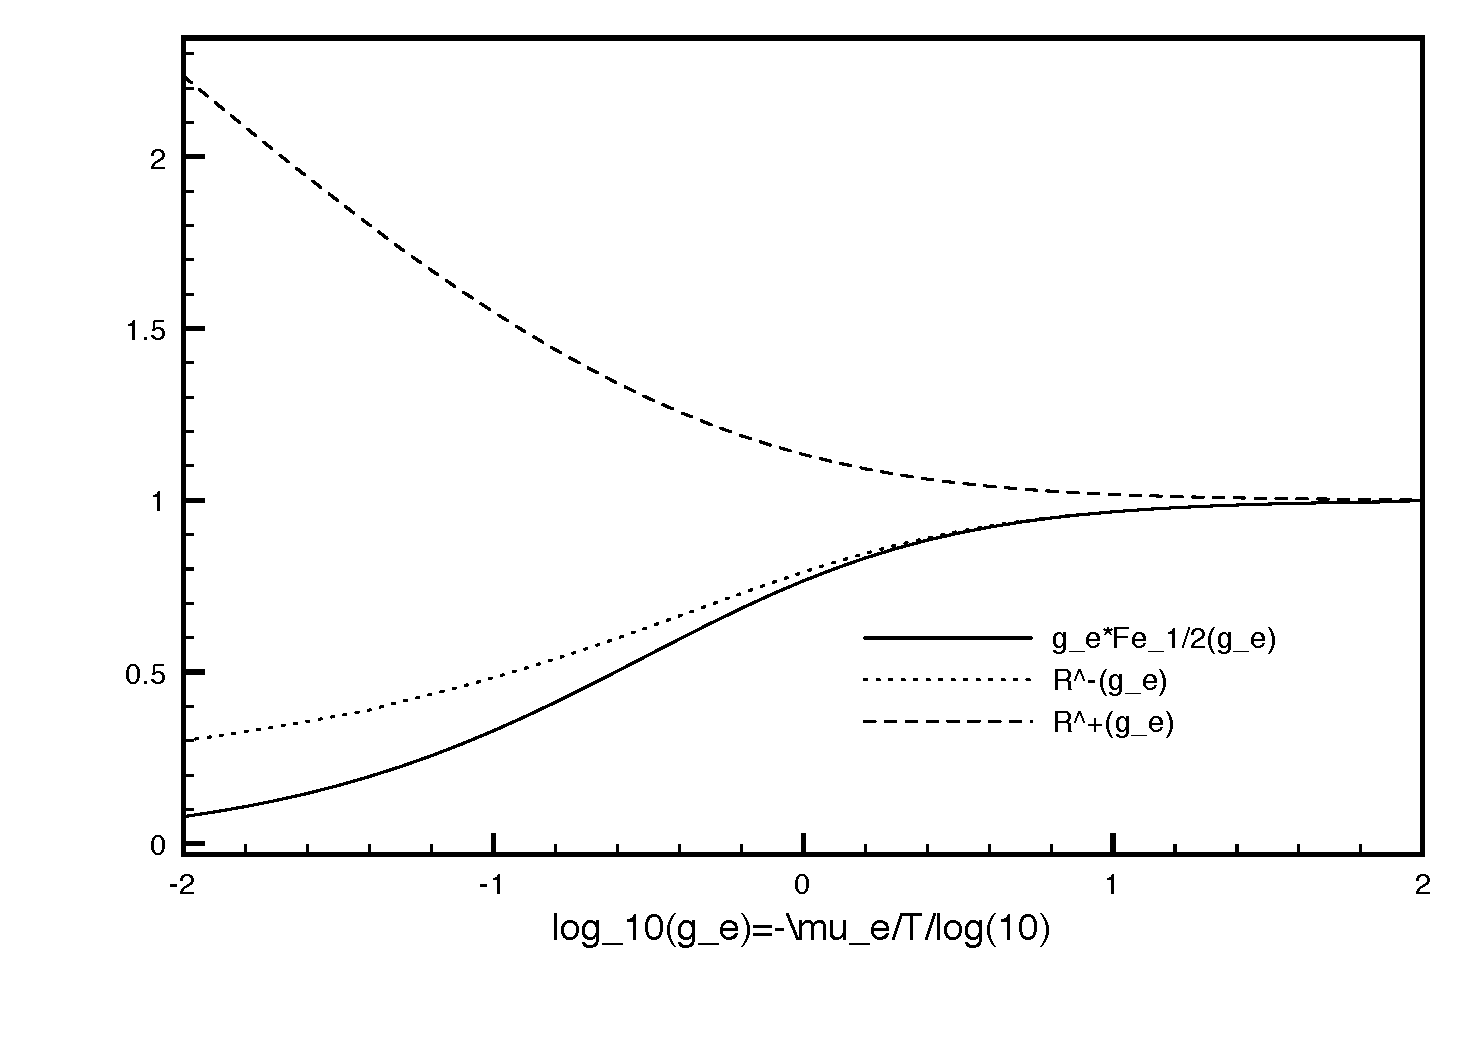
\includegraphics[scale=0.6]{FermiFunction.eps}
\caption{The Fermi function of index 1/2 multiplied by $g_e$ (solid) and the ratio functions (dashed) calculated using the described algorithm.}
\end{figure}


%\section{Appendix B: Partition function and excitation}
{\bf Common properties of mean values and covariances.}
Recall the definition of mean value (also referred to as "expected value"):
\begin{equation}
\langle f_i \rangle = \sum_i p_i f_i.
\end{equation}
Where $p_i$ acts as the probability of occurence of state $i$.
Covariance is constructed using the definition of mean value described above:
\begin{equation}
Cov(a,b) = \langle \delta a \delta b \rangle =
\langle (a - \langle a \rangle) (b - \langle b \rangle) \rangle,
\end{equation}
where $\delta a = a - \langle a \rangle$.
One of the useful properties of covariance is as follows:
\begin{equation}
\langle \delta a \delta b \rangle = \langle ab \rangle - \langle a \rangle \langle b \rangle,
\end{equation}
\begin{eqnarray}
\nonumber proof: \langle (a - \langle a \rangle) (b - \langle b \rangle) \rangle =
\langle ab - a \langle b \rangle - b \langle a \rangle + \langle a \rangle \langle b \rangle \rangle = \\ \nonumber
\langle ab \rangle - 2 \langle a \rangle \langle b \rangle + \langle a \rangle \langle b \rangle =
\langle ab \rangle - \langle a \rangle \langle b \rangle.
\end{eqnarray}
Another property we actually use in the code to optimize the
calculation of covariances is as follows:
\begin{equation}
\langle \delta a \delta b \rangle = \langle (a - \langle a \rangle) b \rangle,
\end{equation}
\begin{equation}
\nonumber proof: \langle \delta a \delta b \rangle =
\langle ab \rangle - \langle a \rangle \langle b \rangle =
\langle ab \rangle - \langle \langle a \rangle b \rangle =
\langle (a - \langle a \rangle) b \rangle.
\end{equation}
Even having no idea about particular properties of either $p_i$ and $f_i$,
one can derive the formula for $d \langle f_i \rangle$ as follows:
\begin{equation}\label{differmean}
d \langle f_i \rangle = \langle \delta f_i \delta \left( \frac{d p_i}{p_i} \right) \rangle +
\langle d f_i \rangle,
\end{equation}
which is useful to calculate partial derivatives of $\langle f_i \rangle$,
for example, $\frac{\partial \langle f_i \rangle}{\partial g_e}$.

Proof:
\begin{eqnarray}
\nonumber d \langle f_i \rangle &=&
d \left( \frac{\sum w_i f_i}{\sum w_i} \right) =
\frac{d(\sum w_i f_i)}{\sum w_i} - \frac{d(\sum w_i) \sum w_i f_i}{\sum w_i} = \\
\nonumber &=& \frac{\sum (w_i df_i + f_i dw_i)}{\sum w_i} - \frac{\sum dw_i}{\sum w_i} \langle f_i \rangle = \\
&=& \langle df_i \rangle + \langle f_i \frac{dw_i}{w_i} \rangle - \langle \frac{dw_i}{w_i} \rangle \langle f_i \rangle =
\langle \delta f_i \delta \left( \frac{dw_i}{w_i} \right) \rangle + \langle df_i \rangle,
\end{eqnarray}
where $w_i = p_i S$ are non-normalized partition functions.




\begin{thebibliography}{99}
\bibitem{ZR}
Ya.B.Zel'dovich and Yu.P.Raizer, Physics of Shock Waves and High Temperature Hydrodynamic Phenomena,
\bibitem{ll}
L.D.Landau and E.M.Lifshitz, Theoretical Physics. Vol.5. Statistical Physics, Part 1. 3rd Edition. Pergamon Press, NY, 1980.
\bibitem{gradshtein}
I.S.Gradshteyn and I.M.Ryzhik, Table of Integrals, Series and Products. Academic Press, NY, 1965.
\bibitem{mcleod}
A.J.MacLeod, Algorithm 779: Fermi-Dirac Functions of Order -1/2, 1/2, 3/2, 5/2. ACM Transactions on Mathematical Software, Vol. 24, No. 1, March 1998.
\bibitem{ionmix}
J.J.MacFarlane.
IONMIX -- a code for computing the equation of state and radiative properties of LTE and non-LTE plasmas.
Computer Physics Communications 56 (1989) 259-278.
\bibitem{drake}
R.P.Drake. High Energy Density Physics. Springer, Berlin-Heidelberg-NY, 2006.
\bibitem{DS}
D.Saltman, Atomic Physics in Hot Plasmas, Oxford University Press US, 1998
\bibitem{AA2}
J.Stein, D.Shalitin, and Akiva Ron. Average-atom models of line broadening in hot dense plasmas.
Physical Review A, Volume 31, Number 1, 1985.
\bibitem{CollisionRadiative}
D.Wunderlich, S.Dietrich, U.Fantz.
Application of a collisional radiative model to atomic hydrogen for diagnosic purposes.
JQS\&RT 110 (2009) 62-71.
\bibitem{CollRad}
J.Yuan, G.A.Moses. YAC: A code using the detailed term accounting model for all-Z elements.
JQS\&RT 99 (2006) 697-711.
\bibitem{EOSTA}
A.Bar-Shalom, J.Oreg, M.Klapisch.
EOSTA -- an improved EOS quantum mechanical model in the STA opacity code.
JQS\&RT 99 (2006) 35-54.
\bibitem{InfernoLike}
B.Wilson, V.Sonnad, P.Sterne, W.Isaacs. PURGATORIO -- a new implementation of the INFERNO algorithm.
JQS\&RT 99 (2006) 658-679.
\bibitem{LineBroadening}
E.Stambulchik, Y.Maron.
A study of ion-dynamics and correlation effects for spectral line broadening in plasma: K-shell lines.
JQS\&RT 99 (2006) 730-749.
\bibitem{LineByZLine}
M.Lino da Silva.
An adaptive line-by-line -- statistical model for fast and accurate spectral simulations in low-pressure plasmas.
JQS\&RT 108 (2007) 106-125.
\bibitem{NonLTEXeSpectrum}
J.Bauche, C.Bauche-Arnoult, O.Peyrusse, A.Bachelier, K.B.Fournier, C.Chenais-Popovics, J.-C.Gauthier
Analysis of a non-LTE xenon spectrum by means of the model of superconfiguration temperatures.
JQS\&RT 81 (2003) 47-55.
\bibitem{Rodriguez0}
R.Rodriguez, J.M.Gil, J.G.Rubiano, R.Florido, P.Martel, E.Minguez.
Relativistic quantum mechanic calculation of photoionization cross-section of hydrogenic and
non-hydrogenic states using analytical potentials.
JQS\&RT 91 (2005) 393-413.
\bibitem{RodriguezPhotoIon}
R.Rodriguez, J.M.Gil, R.Florido.
Photoionization cross section of non-hydrogenic levels for weakly coupled plasmas.
JQS\&RT 108 (2007) 239-255.
\bibitem{STA}
A.Bar-Shalom, J.Oreg, W.H.Goldstein, D.Shvarts, A.Zigler.
Super-transition-arrays: A model for the spectral analysis of hot, dense plasma.
Physical Review A, Volume 40, Number 6, 1989.
\bibitem{StewartPyatt}
J.C.Stewart, K.D.Jr.Pyatt.
Lowering of ionization potentials in plasmas.
Astrophysical Journal, Volume 144, Number 3, p.1203, 1966.
\bibitem{SuperConfiguration}
Jean-Christophe Pain, Thomas Blenski.
Self-consistent approach for the thermodynamics of ions in dense plasmas
in the super configuration approximation.
JQS\&RT 81 (2003) 355-369.
\bibitem{Voight}
Mofreh R.Zaghloul.
Comment on "a fast method of modeling spectral line".
JQS\&RT 109 (2008) 2895-2897.
\bibitem{WireArray}
M.F.Yilmaz, A.S.Safronova, V.L.Kantsyrev, A.A.Esaulov, K.M.Williamson, G.C.Osborne, I.Sherestha, N.D.Ouart.
Spectroscopic features of implisions of Mo single- and double-planar wire arrays produced on the 1 MA Z-pinch generator.
JQS\&RT 109 (2008) 2877-2890.
\bibitem{Xe11}
H.-P.Garnir, S.Enzonga Yoca, P.Quinet, E.Biemont.
Lifetime and transition probability determination in Xe IX.
JQS\&RT 110 (2009) 284-292.
\end{thebibliography}

\end{document}
